\chapter{System Setup}
\label{sec:SystemSetup}

An important contribution of this thesis, was the incorporation of all system's parts in the simulation. By that,  possibly dangerous or unpredicted situations in the real system were avoided by carefully studying the MAV's simulated responses to the experiments. At the beginning of the project, were created some ROS packages so as to obtain the necessary experience and get familiar with the system. All the following packages were written on a computer running on Ubuntu 14.04 LTS alongside with ROS Indigo Igloo\protect\footnotemark. The simulator used in this project is the RotorS simulator from ASL which is based on Gazebo\cite{GazeboSimulator}.

\footnotetext{http://wiki.ros.org/indigo}

Now follows the description of the ROS packages that were created for this project, some packets with very similar role and structure are omitted from the description. All the  packages are written in the C\texttt{++} programming language\cite{Stroustrup} and can be accessed at the ASL's GitHub page under the repository mav\textunderscore demos\cite{MyRepoGitHub}. 


\section{Connecting the Camera with ROS}
\label{sec:connectedCamera}
The very first task was to connect a camera to the ROS so as to obtain the images of the markers. The camera chosen for this project was the Logitech Tessar HD, for its calibration and image rectification the ROS camera\textunderscore calibration package and the image \textunderscore proc node were used respectively. After the camera setup, the detection of the Apriltags\cite{olson2011tags} came into focus. In order to detect the position and orientation of the aforementioned, the apriltag\textunderscore ros package was used. This provides a ROS wrapper for the C\texttt{++} library\cite{ROSApriltag}. It should be mentioned that although this library detects position very accurately it faces some problems with the detection of the marker's orientation. The problem becomes worse as the distance between the camera and the target increases. 



\section{Moving the Simulated MAV}
\label{sec:movingMAV}
After the camera setup, the main focus moved towards connecting the Apriltag detection with the simulated MAV. This was conducted in the mav\textunderscore demo\textunderscore camera package. In there, two nodes are created, except of course those referring to camera, one that detects the Apriltag and publishes the detection data to a ROS topic and another one that conducts the motion. In this specific example the user moves the tag in front of the camera and the simulated MAV moves accordingly. It should be noted, that in this example the MAV does not detect the marker, its motion is based on the detection from the USB camera. As can be seen from figure \ref{pics:mav_demo_camera} when the package is ran, two windows are created, one depicting the detections from the USB camera, for the user to know whether or not the marker is detected and the simulator's window with the moving MAV.  

For safety reasons, the position of the MAV in the z axis is augmented by 50 cm. Thus, when the user holds the marker at the same height as the camera, the MAV does not collide with the ground.

\begin{figure}
   \centering
   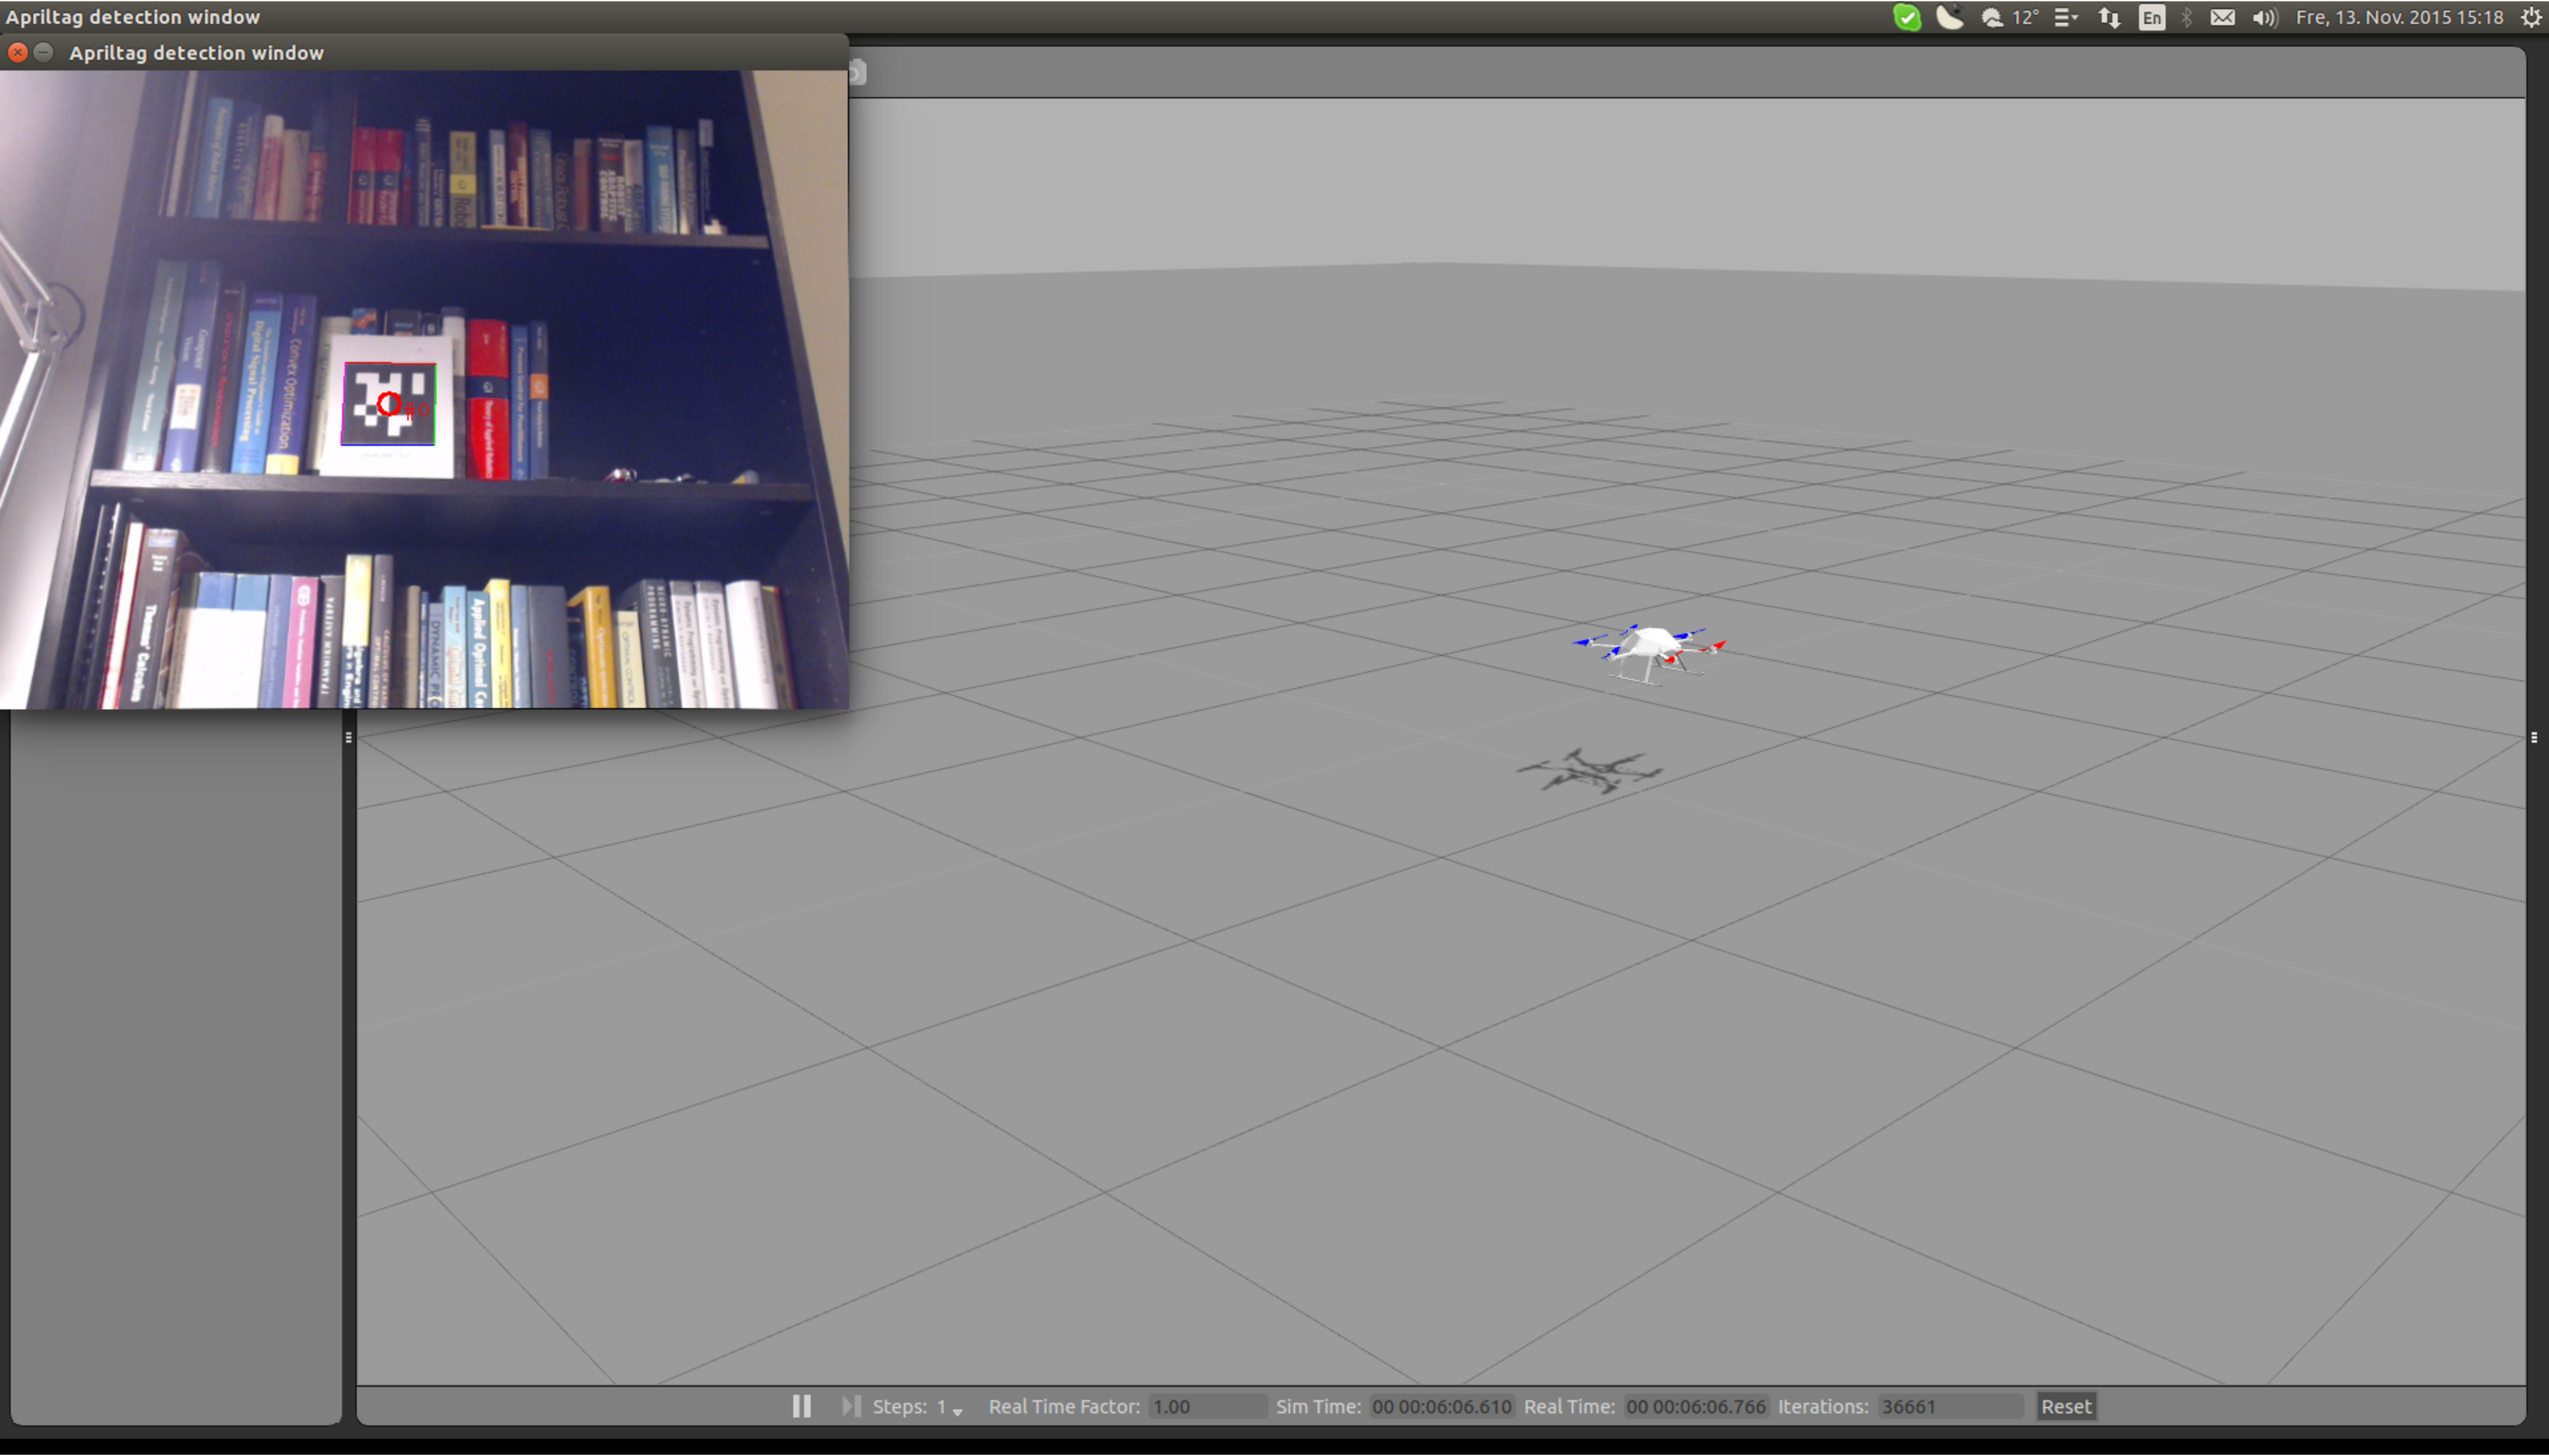
\includegraphics[width=0.75\textwidth]{images/mav_demo_camera.pdf}
   \caption{The MAV moves based on the detection of the USB camera}
   \label{pics:mav_demo_camera}
\end{figure}


\section{Creating the Apriltag Models}
\label{sec:cubeRobots}

In order to make the simulation realistic, the MAV should detect the Apriltags by its own camera, in the simulated world. Thus, models representing the various tags were needed. The objects were simple cuboids which had as texture the Apriltag's image. It should be mentioned that the dimensions (width and height) of the cuboids should be identical as the parameters passed from the ROS parameter server to the detection node, so as to get the correct position estimation. Furthermore, the third dimension of the cuboid (length) should be kept minimal so as to avoid fallacious detections during the turning of the MAV.

\section{Realistic Simulation Scenarios}
\label{sec: apriltagFireflySimulation}

Before moving to the real system, some more realistic simulation scenari were implemented so as to study the MAV's behavior under various circumstances. In this case the user inserts different markers inside the simulated world and the MAV performs a variety of motions with respect to the different detected markers. In order to distinguish between the various markers, we use the id of each tag. It should be mentioned, that at each time only one Apriltag should be detected from the MAV's sensor so as to have a smooth operation.

\begin{figure}
   \centering
   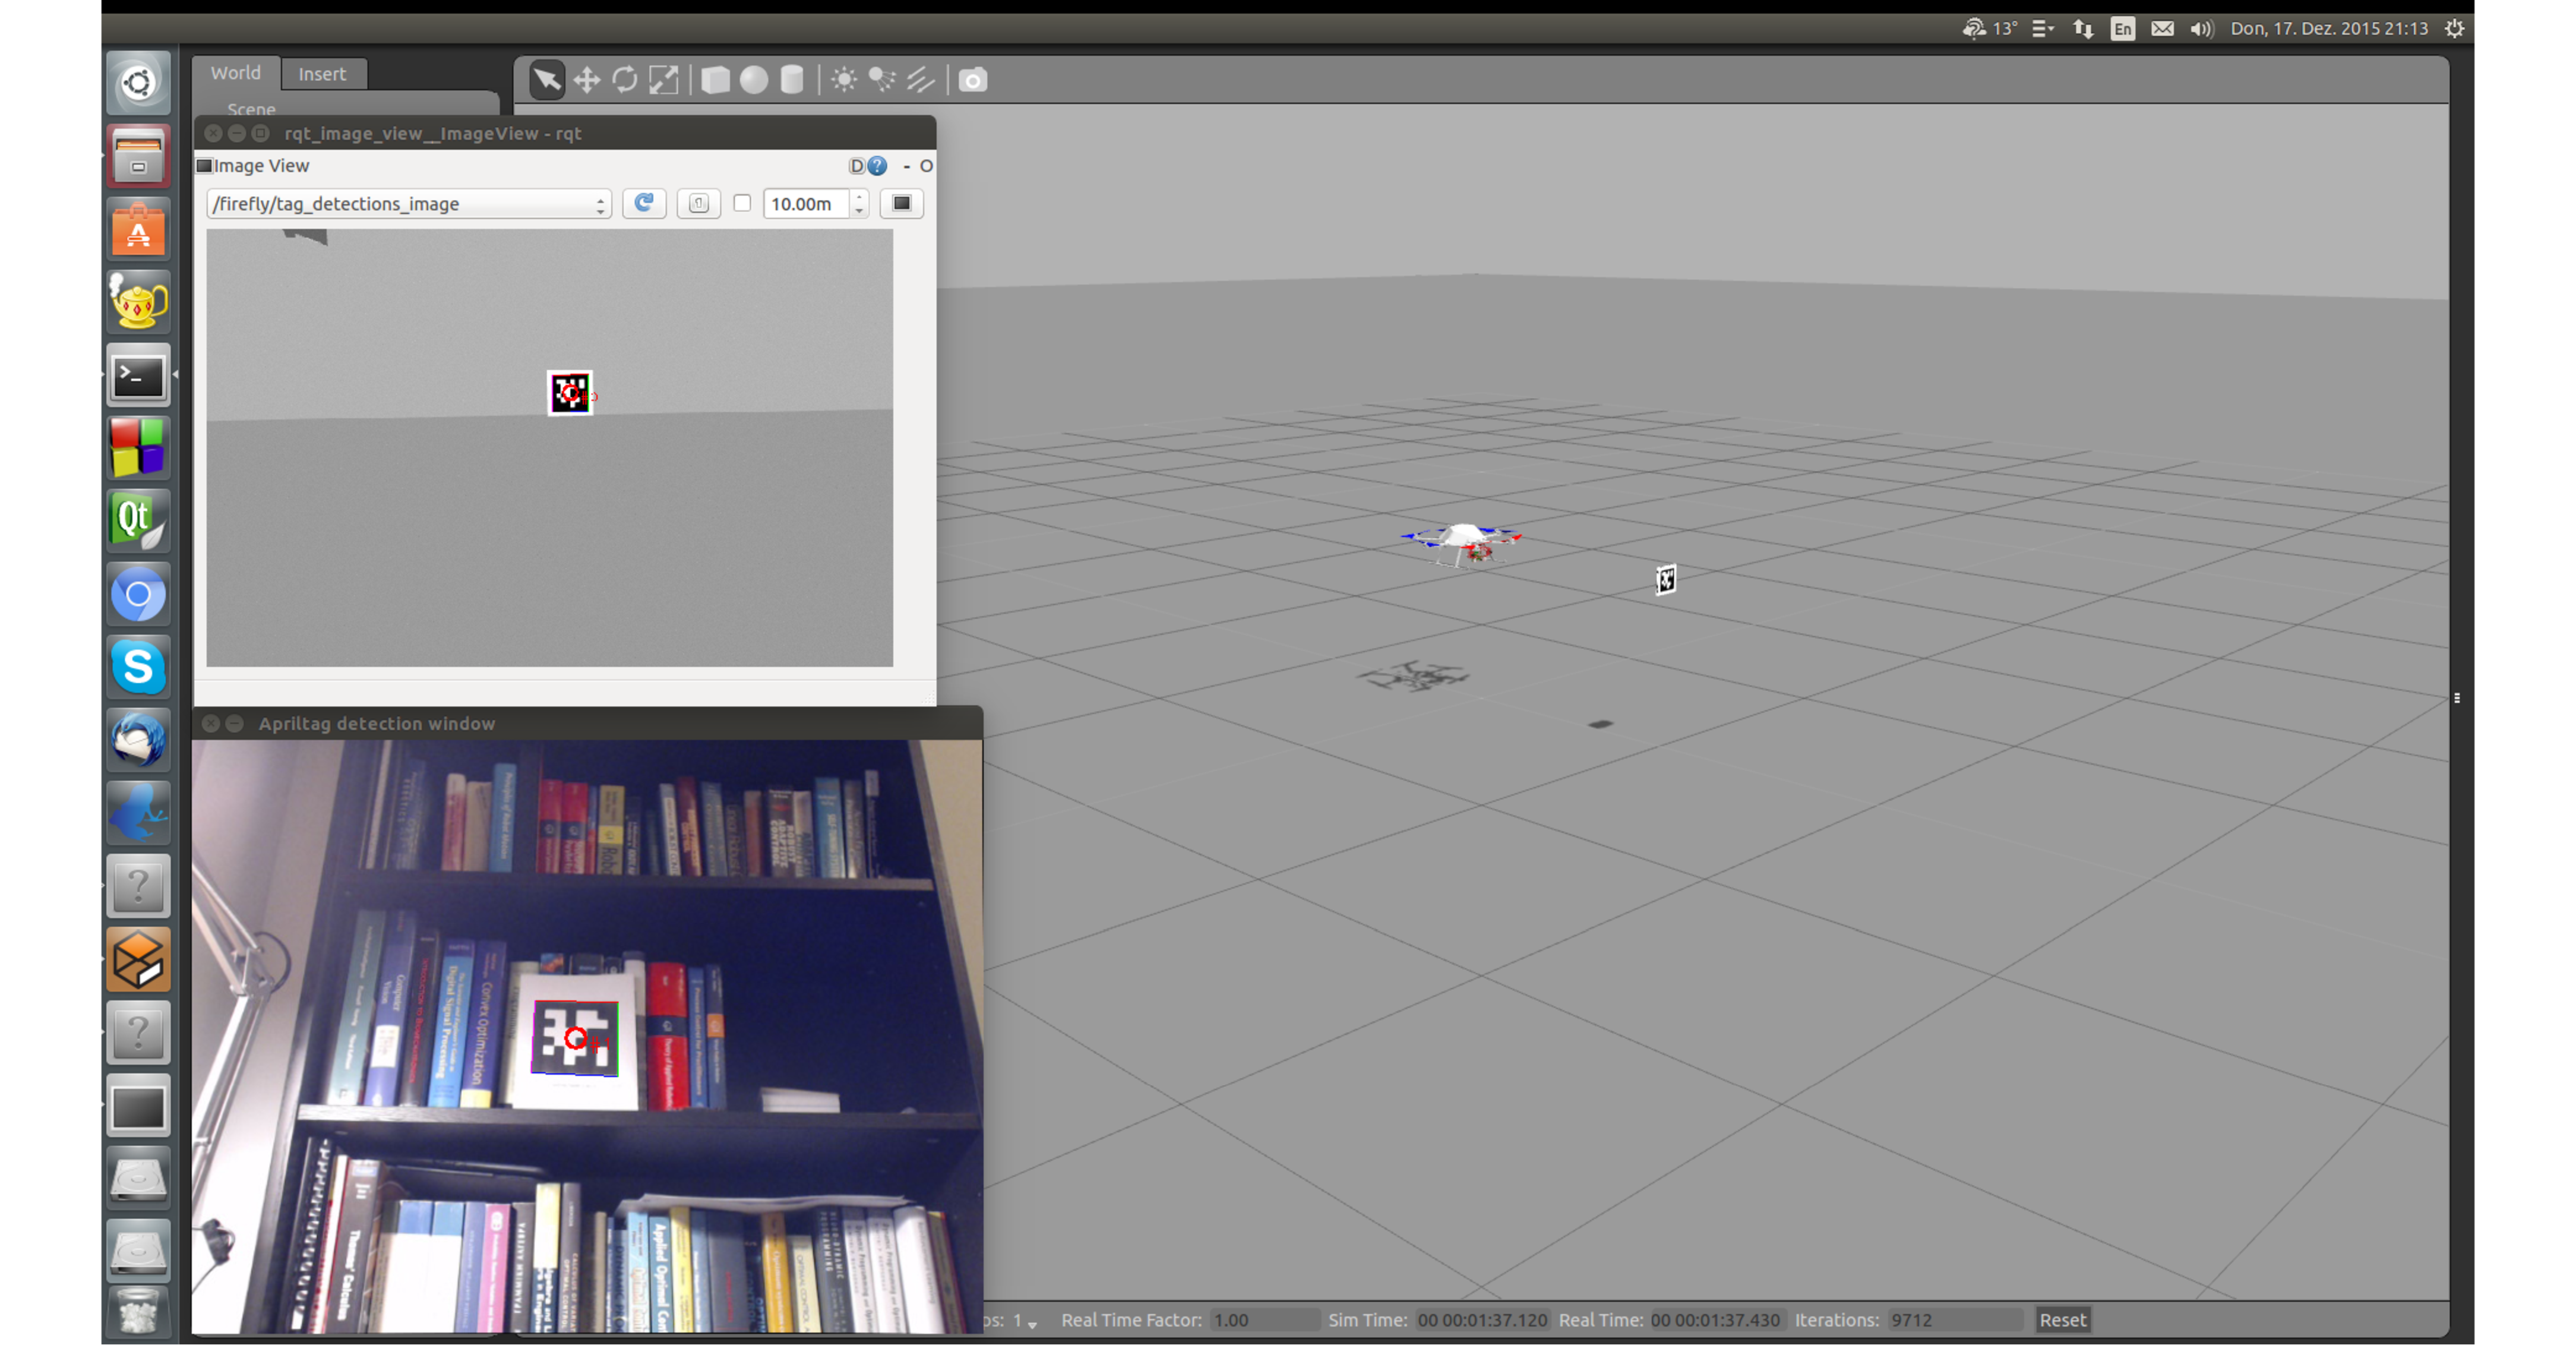
\includegraphics[width=0.98\textwidth]{images/sim_atag_mavdet_win.pdf}
   \caption{Realistic simulated scenario.}
   \label{pics:apriltags_firefly_simulation_screen}
\end{figure}

The default motion, consists of the user moving a marker in front of the computer's camera which controls the pose of the Apriltag marker in the simulation. The MAV is programmed to follow the marker, by having adequate distance so as to guarantee the user's safety in the real world system. The predefined safety distance is set by the user at a configuration file that provides the system with various constant parameters. In the case that the program cannot find the configuration files for some reason, it sets the aforementioned values to predefined thresholds so as to guarantee the user's and system's safety. 

Furthermore, the MAV is capable of performing take-offs and landings whenever the user wants. When the user wants to land the MAV, he just has to present a specific marker in front of the camera. The exact same procedure, but with a different marker, is followed to make the MAV hovering again. The program stores the last x,y and z coordinates along with the last orientation of The MAV before the landing command. It should be mentioned that in order to switch from landing state back to following the tag state the user must show to the MAV a specific marker that triggers a reset state. In this reset state, the MAV goes back to its starting position and height, just as before its landing. Furthermore, it is assumed that throughout the simulation the MAV's inertial measurement frame is assumed to be initialized relative to the ground.

\begin{figure}
   \centering
   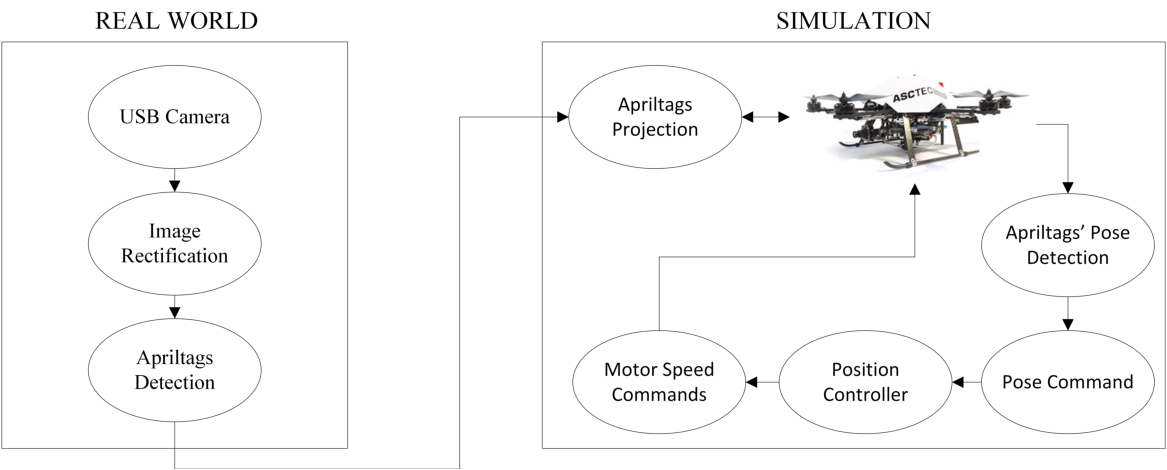
\includegraphics[width=0.98\textwidth]{images/cam_firefly_sim.pdf}
   \caption{Approximation of nodes running in the simulation \protect\footnotemark }
   \label{pics:mav_demo_camera_rosgraph}
\end{figure}

\footnotetext{The Firefly's image was taken from http://www.asctec.de/en}
A screenshot describing the operation of the MAV during the realistic scenari is provided at the figure \ref{pics:apriltags_firefly_simulation_screen}. Here we can see, the detection of the Apriltag in the real world, at the lower left window, the marker as detected from the MAV's camera into the simulated world, in the upper left window, and finally the MAV and the Apriltag in the simulated world. Furthermore, in figure \ref{pics:mav_demo_camera_rosgraph} there is a graphic approximation of the running nodes, which explains the underlying procedures. In other words, the marker is detected in the real world from the USB camera, and the detected pose commands the position and orientation of the simulated Apriltag. Then, the simulated MAV detects the marker from its own camera and sends the desired pose based on its detection to the position controller. 

